\subsection{Random Forest}

\begin{itemize}
\item
  \emph{\textbf{Introduction to Random Forest}}: Random forest is a
  machine learning technique that has gained widespread popularity for
  their versatility and effectiveness in various prediction tasks
  (Breiman 2001, Epifanio 2017). This approach, which comprises an
  ensemble of decision trees and seamlessly integrates feature selection
  and interactions into the learning process, is highly favored by
  researchers and practitioners alike (Breiman 2001, Brieuc et al. 2018,
  Fabris et al 2018). Random forests have been successfully applied
  across diverse domains such as posttranslational modification site
  prediction, fold recognition, protein-protein interaction site
  prediction, enzyme function classification, and interaction or
  association between molecular markers and phenotype (Fraimout et al.
  2017, Brieuc et al. 2018, Fabris et al 2018).
\item
  \textbf{Technical overview of random forest:}
\end{itemize}

\begin{quote}
\textbf{Description of Random Forest:} Random Forest is a versatile and
powerful machine learning algorithm used for both classification and
regression tasks (Breiman 2001). It belongs to the ensemble learning
family, which combines multiple individual models to improve overall
predictive performance. The "forest" in Random Forest is composed of a
collection of decision trees.
\end{quote}

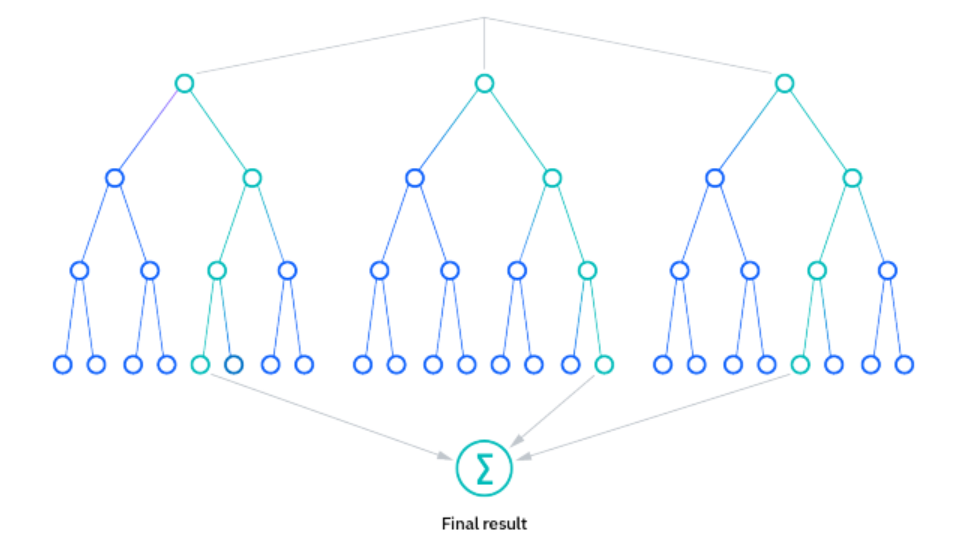
\includegraphics[width=3.02722in,height=1.71542in]{figs/rf.png}

\begin{enumerate}
\def\labelenumi{\alph{enumi}.}
\item
  \textbf{Decision Trees:} Each tree in the forest is a decision tree,
  which is a flowchart-like structure where an internal node represents
  a feature or attribute, the branch represents a decision rule, and
  each leaf node represents the outcome. Decision trees are simple yet
  effective models for classification and regression (Hastie et al.
  2009).
\end{enumerate}

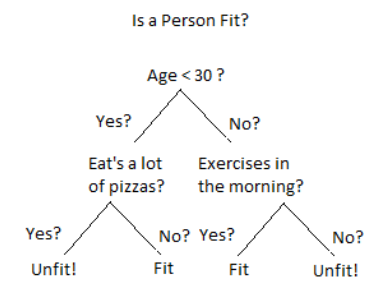
\includegraphics[width=2.22832in,height=1.69421in]{figs/tree.png}

\begin{enumerate}
\def\labelenumi{\alph{enumi}.}
\setcounter{enumi}{1}
\item
  \textbf{Randomness:} Random Forest introduces randomness in two key
  ways (Breiman 2001):

  \begin{itemize}
  \item
    Random Sampling: During the training phase, instead of using the
    entire dataset to build each tree, Random Forest randomly selects a
    subset of the data (with replacement), known as bootstrap samples.
  \item
    Random Feature Selection: At each node of the decision tree, instead
    of considering all features to determine the best split, Random
    Forest randomly selects a subset of features. This introduces
    diversity among the trees and prevents overfitting.
  \end{itemize}
\item
  \textbf{Voting or Averaging:} For classification tasks, Random Forest
  combines the predictions of all the individual trees by majority
  voting, i.e., the class that receives the most votes. For regression
  tasks, it averages the predictions made by all the trees to obtain the
  final prediction (Breiman L. 2001).
\end{enumerate}

\begin{itemize}
\item
  \textbf{Training Techniques and Optimization Algorithms:}

  \begin{enumerate}
  \item
    Bootstrap Aggregating (Bagging): Random Forest employs a technique
    called bagging, which involves training each decision tree on a
    random subset of the training data with replacement. This helps in
    reducing overfitting by introducing diversity among the trees.
  \item
    Decision Tree Construction: Each decision tree in the Random Forest
    is constructed using a subset of features selected randomly at each
    node. This randomness ensures that the trees are less correlated
    with each other, leading to a more robust model.
  \item
    Number of Trees (n\_estimators): One of the hyperparameters of
    Random Forest is the number of trees in the forest. Typically,
    increasing the number of trees improves performance, but it also
    increases computational cost. Finding the optimal number of trees
    often involves cross-validation techniques.
  \item
    Feature Importance: Random Forest provides a measure of feature
    importance, which indicates the contribution of each feature in
    predicting the target variable. This information can be useful for
    feature selection and understanding the underlying data.
  \item
    Parallelization: Training each decision tree in Random Forest is
    independent of the others, making it highly parallelizable. Many
    implementations of Random Forest leverage parallel computing to
    speed up the training process, especially when dealing with large
    datasets.
  \item
    Hyperparameter Tuning: Random Forest has several hyperparameters
    such as the number of features to consider at each split, maximum
    depth of the trees, minimum samples per leaf, etc. Grid search or
    randomized search techniques can be used to find the optimal
    combination of hyperparameters (Hastie et al. 2009).
  \end{enumerate}
\end{itemize}

\begin{itemize}
\item
  \textbf{Usage in biological research}.
\end{itemize}

\begin{quote}
\textbf{Case 1:} A practical introduction to random forest for genetic
association studies in ecology and evolution.. In case 1, they used R.
They were looking at the association between molecular markers and
phenotype.

\textbf{Case 2:} a new approach for interpretation random forest models
and its application to the biology of aging. In case 2, they used Linux
Mint. They were trying to predict the expression of genes in brain
aging.
\end{quote}

\begin{itemize}
\item
  \textbf{Implementation details}:
\end{itemize}

\begin{quote}
\textbf{Case 1}: In this study, they explore the use of Random Forest
(RF) to discern loci underlying both discrete and quantitative traits,
particularly when studying wild or nonmodel organisms. RF is becoming
increasingly used in ecological and population genetics because, unlike
traditional methods, it can efficiently analyze thousands of loci
simultaneously and account for nonadditive interactions. They described
to prepare data for RF, including initial data exploration and the
identification of important covariates and possible confounding factors.
They next provide guidance on the initiation of RF and the optimization
of the algorithm parameters for classification and regression. Last,
they summarize methods for interpreting the results of RF and
identifying trait-associated, or predictor, loci (Fabris et al 2018).

\textbf{Case 2}: In this study, the authors were looking at how we can
use RF to predict when a gene is being over expressed, under expressed
or has no change in the brain when aging. The author use Linux Mint. To
look for the association of gene expression and aging, the author
created a dataset with different type of gene that are improved in
aging. Following that, the author evaluated the precise accuracy using
the Area Under the Receiver Operating Characteristic curve (AUROC),
computed via 10-fold cross-validation. AUROC values indicate the model's
performance, with 1.0 representing perfect classification. 10-fold
cross-validation is utilized for AUROC calculation, with the mean value
obtained over 30 runs for stability. Internal 5-fold cross-validation
optimizes RF parameters, mtry and nTree, within each fold of external
cross-validation. Dataset imbalance towards the class 'no change in
expression (N)' prompts under-sampling to balance class distribution,
thereby enhancing model performance. Feature importance is assessed
using the 'Computing the Predictive Accuracy of Random Tree Rules with
Positive (±) Feature Values' (COMPACT + FV) Algorithm. This algorithm
focuses on IF-THEN rules containing positive feature values and utilizes
Out-Of-Bag (OOB) instances to compute statistics, such as OOB coverage
and OOB hits, for each feature and class. Upon algorithm execution,
importance scores for every feature and class in the RF are computed,
with precision calculated for rules containing positive feature values
predicting each class (Brieuc et al. 2018).
\end{quote}

\subsubsection{Implementation of Random Forest Algorithm}

\begin{algorithm}
    \caption{Python RF example using \texttt{sklearn}}\label{alg:rf_py}
\begin{lstlisting}[language=Python]
rf_model = RandomForestClassifier(n_estimators=100, criterion='gini',
max_depth=None, min_samples_split=2, min_samples_leaf=1,
max_features='auto', bootstrap=True, class_weight='balanced')

rf_model.fit(X_train, y_train)
rf_pred = rf_model.predict(X_test)

\end{lstlisting}
\end{algorithm}

\begin{algorithm}
    \caption{R RF example using \texttt{foobar}} \label{alg:rf_r}
\begin{lstlisting}[language=R]
rf_model <- randomForest(x = X_train, y = y_train, ntree =
100, importance = TRUE, classwt = "balanced")

rf_pred <- predict(rf_model, X_test)
\end{lstlisting}
\end{algorithm}

\subsubsection{Challenges and considerations of Random Forest Model in Biological Contexts}

\begin{enumerate}
\item
  Overfitting: While Random Forest is robust against overfitting
  compared to individual decision trees, it can still occur, especially
  with noisy or high-dimensional biological data. Careful tuning of
  hyperparameters such as the number of trees, maximum depth, and
  minimum samples per leaf is necessary to mitigate overfitting and
  ensure generalization to unseen data.
\item
  Data Requirements: Random Forest performs well with large datasets,
  but biological datasets often pose unique challenges such as
  imbalanced class distributions, missing values, and high
  dimensionality. Preprocessing steps like feature selection,
  imputation, and data balancing are crucial to optimize model
  performance and prevent biases in genetic association studies.
\item
  Model Complexity: Random Forest can handle complex relationships
  between genetic variables and phenotypic traits, but it may not
  capture subtle interactions or nonlinearities present in biological
  systems. Model interpretation and validation techniques, such as
  permutation importance and partial dependence plots, help elucidate
  the relationships between genetic predictors and ecological or
  evolutionary outcomes.
\item
  Validation and Generalization: Assessing the performance and
  generalization of Random Forest models across different populations,
  species, or environmental conditions is essential in biological
  studies. Cross-validation techniques, independent validation datasets,
  and robustness testing help ensure the reliability and applicability
  of Random Forest models in diverse ecological and evolutionary
  contexts.
\end{enumerate}

\subsubsection{Impact and future perspective}

  \begin{itemize}
  \item
    \emph{Impact}: the ability of the Random Forests approach to
    handle complex data and produce robust predictions makes it a go-to
    choice for tackling challenging problems in bioinformatics and
    beyond. In biology specifically, RF can be used to analyze large
    datasets, which include, but are not limited to, evolution,
    molecular biology, phylogenetics, phylogenomics, and even the
    biology of aging (Touw et al. 2012).
  \item
    \emph{Future perspective}: currently and in the near future, we
    can continue to use RFs to test and work with big datasets that
    various omics approaches (e.g., genomics, proteomics, metabolomics)
    provide. This allows us to study how different variables (e.g.,
    genes, temperatures, alleles) are associated with various organisms
    (e.g., humans, plants, animals). Furthermore, we can assess how
    different diseases impact different groups (Touw et al. 2012).
  \end{itemize}


TODO: migrate these to bibtex and update actual refs
  \textbf{References}

  \begin{itemize}
  \item
    \textbf{Brieuc et al. 2018}. A practical introduction to random
    forest for genetic association studies in ecology and evolution.
    Molecular Ecology Resources.
  \item
    \textbf{Fraimout et al. 2017}. Deciphering the routes of invasion od
    Drosophila suzikii by means of ABC Random Forest. Molecular Biology
    and Evolution.
  \item
    \textbf{Fabris et al. 2018}. A new approach for interpretation
    random forest models and its application to the biology of aging.
    Bioinformatics.
  \item
    \textbf{Breiman} L\textbf{. 2001.} Random forests. Mach Learn. 2001;
    45(1):5--32.
  \item
    \textbf{Epifanio 2017}. Intervention in prediction meausure: a new
    approach to assessing variable importance for random forests.
  \item
    \textbf{Hastie et al. 2009.} The elements of statistical learning:
    data mining, inference, and prediction. Springer Science \& Business
    Media.
  \item
    \textbf{Touw et al. 2012.} Data mining in the Life Sciences with
    Random Forest: a walk in the park or lost in the jungle? Briefings
    in Bioinformatics
  \end{itemize}
